\newpage
\mychapter{Результаты исследования}

Основная проблема, возникающая при вращении спина в NV-центре --
недостаточно большой коэффициент взаимодействия поля со спином,
влекущий высокую длительность операции. С другой стороны, увеличение
этого коэффициента (за счет увеличения амплитуды поля) приводит к
высокой паразитной заселенности не используемого спинового
подуровня. Нахождение оптимального поля в такой ситуации явилось бы
очень полезным результатом.
\section{Аналитическое решение}
Произведем расчет в двухуровневом приближении при малых
амплитудах поля. Для этого переведем гамильтониан
(\ref{eq:shamiltonian}) в матричную форму:
\[  \hat{H}_{NV} = \frac{1}{2} \left( 
  \begin{array}{ccc}
    \hbar D + \sqrt{2} g_e \mu_B B_z &
    \sqrt{2} g_e \mu_B B_0(t) cos(\omega t) & 
    2 \hbar E\\
    \sqrt{2} g_e \mu_B B_0(t)t cos(\omega t) & 
    0 & 
    \sqrt{2} g_e \mu_B B_0(t) cos(\omega t) \\
    2 \hbar E & 
    \sqrt{2} g_e \mu_B B_0(t) cos(\omega t) & 
    \hbar D - \sqrt{2} g_e \mu_B B_z
  \end{array} \right)
\]

Волновая функция NV-центра: $|\Psi\!>~= C_{-1}|\!-\!1\!> +~C_{0}|0\!> +~C_{1}|1\!>$
Решая уравнение Шредингера: $i \hbar
\frac{\partial}{\partial t}|\Psi> = \hat{H}_{NV}|\Psi>$, и выбрав
частоту микроволнового поля $\omega$ равной частоте перехода между $|0\!>$
и $|\!-\!1\!>$, получаем
систему из трех уравнений:
\begin{equation*}
\begin{cases} 
  i \hbar \dot{C}_{0} = \frac{C_{-1}}{2 \sqrt{2}} g_e \mu_B B_0(t)
  \{e^{-2it\omega_{-1}} + 1 \} + \frac{C_1}{2 \sqrt{2}} g_e \mu_B B_0(t)
  \{e^{-it(\omega_1 + \omega_{-1})} + e^{-it(\omega_1 - \omega_{-1})} \}\\ 
  i \hbar \dot{C}_1 = C_{-1} \hbar E e^{-it(\omega_{-1} - \omega_1)} + \frac{C_0}{2 \sqrt{2}} g_e \mu_B
  B_0(t) \{ e^{-it(\omega_{-1} - \omega_1)} + e^{it(\omega_{-1} + \omega_1)} \} \\ 
  i \hbar \dot{C}_{-1} = C_1 \hbar E e^{-it(\omega_1 - \omega_{-1})} +
  \frac{C_0}{2 \sqrt{2}} g_e \mu_B B_0(t) \{ e^{-2it\omega_{-1}} + 1 \} 
\end{cases},
\end{equation*}
где приняты обозначения: $\omega_{-1} = D - \frac{g_e \mu_B B_z}{\hbar}$ -- частота перехода $|0\!> \to |1\!>$,
$\omega_{1} = D + \frac{g_e \mu_B B_z}{\hbar}$ -- частота перехода $|0\!> \to |\!-\!1\!>$.

В приближении вращающейся волны коэффициент взаимодействия
микроволного поля с NV-центром $g \approx \mu_B B_0$ много меньше
величины расщепления уровней $\Delta \approx \mu_B B_z$. В таком
случае можно
считать, что $\omega_1 >> \omega_{-1}$. Тогда система сводится к системе из двух уравнений:
\begin{equation*}
\begin{cases} 
  i \hbar \dot{C}_0 = \frac{C_{-1}}{2 \sqrt{2}} g_e \mu_B
  B_0(t) ( 1 + e^{-2 i \omega_{-1} t} )\\
  i \hbar \dot{C}_{-1} = \frac{C_0}{2 \sqrt{2}} g_e \mu_B B_0(t) ( 1 +
  e^{2 i \omega_{-1}t})\\
\end{cases}.
\end{equation*}
%% Решение полученной системы уравнений имеет вид:\\
%% \begin{equation*}
%% \begin{cases}
%% C_0 = A\cdot e^{(\int \limits_{1}^{t} \frac{i g_e \mu_B B_0(\xi)}{2 \sqrt{2}
%% \hbar} d\xi)} + B\cdot e^{(-\int \limits_{1}^{t} \frac{i g_e \mu_B
%%     B_0(\xi)}{2 \sqrt{2} \hbar} d\xi)}\\
%% C_{-1} = A\cdot e^{(\int \limits_{1}^{t} \frac{i g_e \mu_B
%%     B_0(\xi)}{2 \sqrt{2} \hbar} d\xi)} + B\cdot e^{(- \int
%%   \limits_{1}^{t} \frac{i g_e \mu_B B_0(\xi)}{2 \sqrt{2} \hbar} d\xi)}\\
%% \end{cases},
%% \end{equation}
%% где константы A и B должны удовлетворять нормировке $|C_0|^2 + |C_1|^2
%% = 1$ и определяются начальными условиями, например $|\Psi_0> = |0\!>$.

Численным решением этой системы был получен график эволюции
заселенностей уровней NV-центра (\ref{fig:two_level}). График построен
при условии, что амплитуда постоянного поля равна 850 Гс, а амплитуда
переменного -- 10 Гс. График функций
имеет вид синусоид.
\begin{figure}[H]\centering
  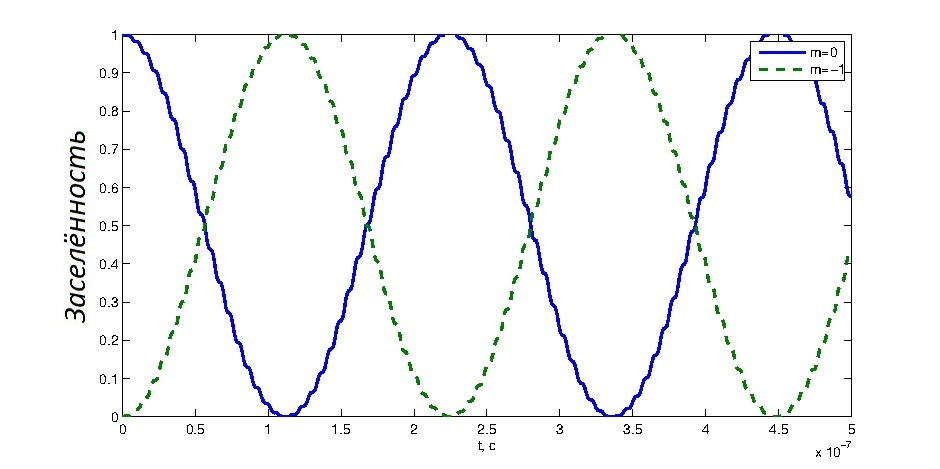
\includegraphics[width=1.1\textwidth,height=0.7\textwidth]{two_level}
  \caption{Эволюция заселенностей уровней NV-центра в двухуровневом приближении.}\label{fig:two_level}
\end{figure}


\section{Компьютерное моделирование}
Для моделирования трехуровневой системы и получения графиков была
написана программа (\ref{code}) с использованием языка программирования
Matlab. Постоянное магнитное поле заданной амплитуды направлено вдоль
оси Z и используется для расщепления по энергии уровней с проекцией
спина, равной $m$=$\pm1$. Было проведено исследование эволюции
заселенностей уровней NV-центра при различных значениях постоянного
поля (\ref{fig:spectrum}), а также различных частотах Раби.
\begin{figure}[H]\centering
  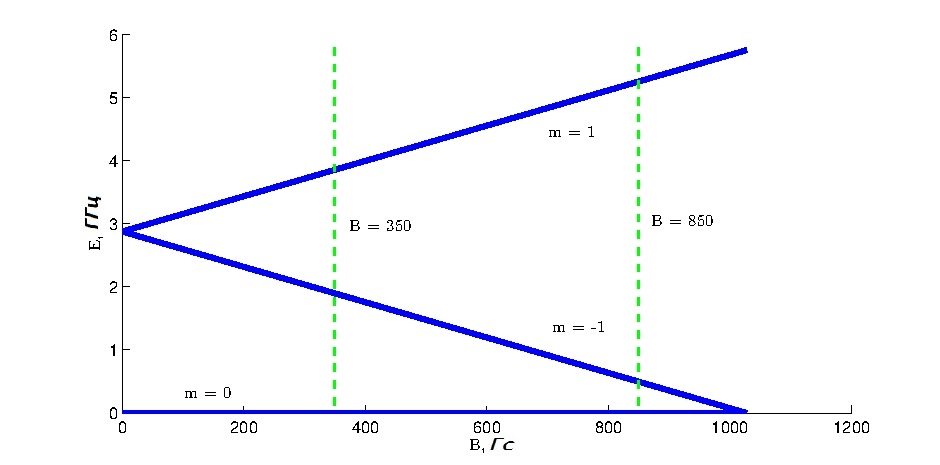
\includegraphics[width=1.1\textwidth,height=0.7\textwidth]{spectrum}
  \caption{Расщепление уровней NV-центра в магнитном поле.}\label{fig:spectrum}
\end{figure}

Прежде всего был произведен расчет в условиях, когда можно применить
приближение вращающейся волны. При амплитуде постоянного поля 350 Гс,
когда амплитуда переменного -- 30 Гс (\ref{fig:350_30}), и при
амплитуде постоянного поля 850 Гс, и амплитуде переменного 20 Гс
соответственно (\ref{fig:850_20}). Вычисления в таких условиях дадут
возможность судить о применимости аналитического решения. Из графиков
видно, что при малых частотах Раби, эволюция заселенностей уровней
NV-центра достаточно хорошо описывается двухуровневым
приближением. Паразитная заселенность уровня с $m_s$=$-1$ пренебрежимо
мала по сравнению с полезными заселенностями.
\begin{figure}[h!]\centering
  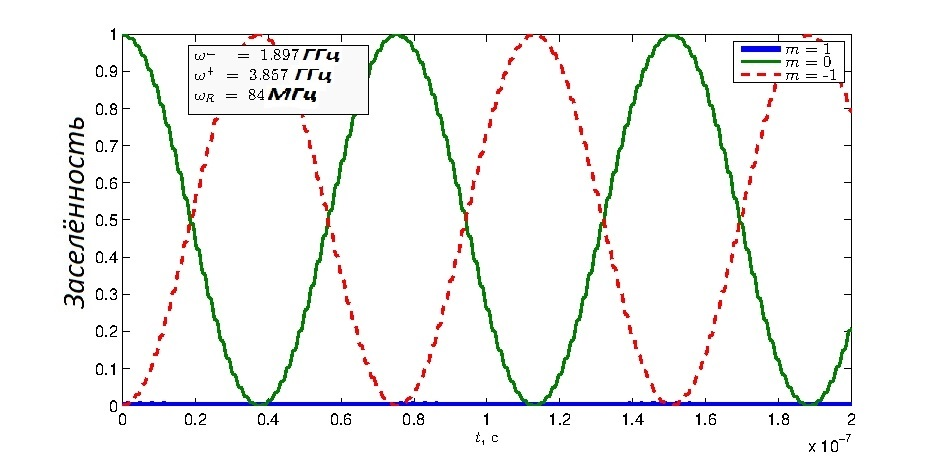
\includegraphics[width=1.1\textwidth,height=0.65\textwidth]{350_30}
  \caption{Эволюция заселенностей уровней NV-центра.}\label{fig:350_30}
\end{figure}
\begin{figure}[h!]\centering
  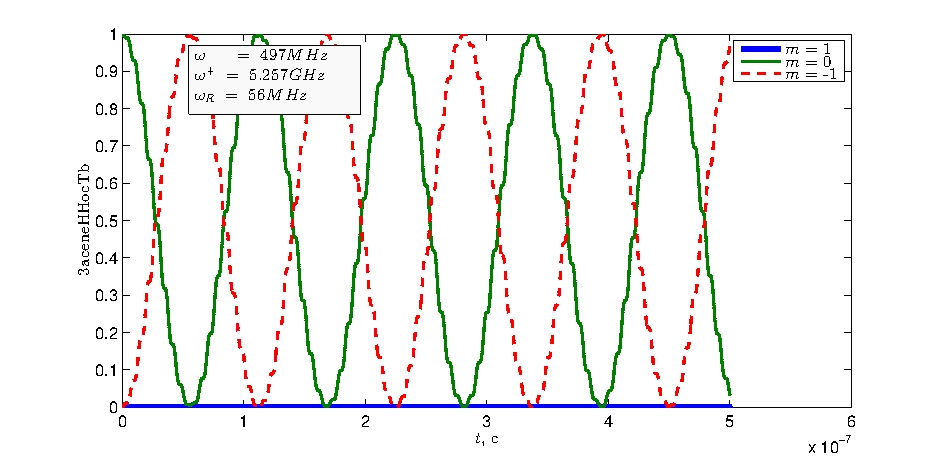
\includegraphics[width=1.1\textwidth,height=0.63\textwidth]{850_20}
  \caption{Эволюция заселенностей уровней NV-центра.}\label{fig:850_20}
\end{figure}

Если увеличивать частоту Раби, нарушая тем самым приближение
вращающейся волны, можно пронаблюдать поведение NV-центра, которое
нельзя получить из аналитических расчетов. Например, на графиках
(\ref{fig:350_100}) (постоянное поле 350 Гс, переменное 100 Гс) и
(\ref{fig:850_150}) (постоянное поле 850 Гс, переменное 150 Гс)
отчетливо видна паразитная заселенность уровня с проекцией спина
$m_s$=$-1$.

На графиках (\ref{fig:350_100}) - (\ref{fig:850_680}) отчетливо видны
``ступеньки'' и с увеличением частоты Раби эти ступеньки становятся
крупнее. Эти ступеньки свидетельствуют о том, что нарушается
приближение вращающейся волны.
\begin{figure}[h!]\centering
  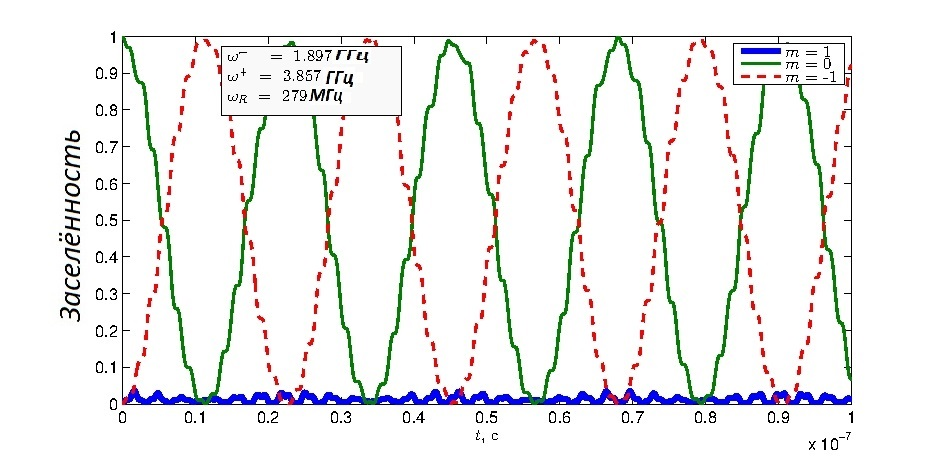
\includegraphics[width=1.1\textwidth,height=0.67\textwidth]{350_100}
  \caption{Эволюция заселенностей уровней NV-центра.}\label{fig:350_100}
\end{figure}
\begin{figure}[h!]\centering
  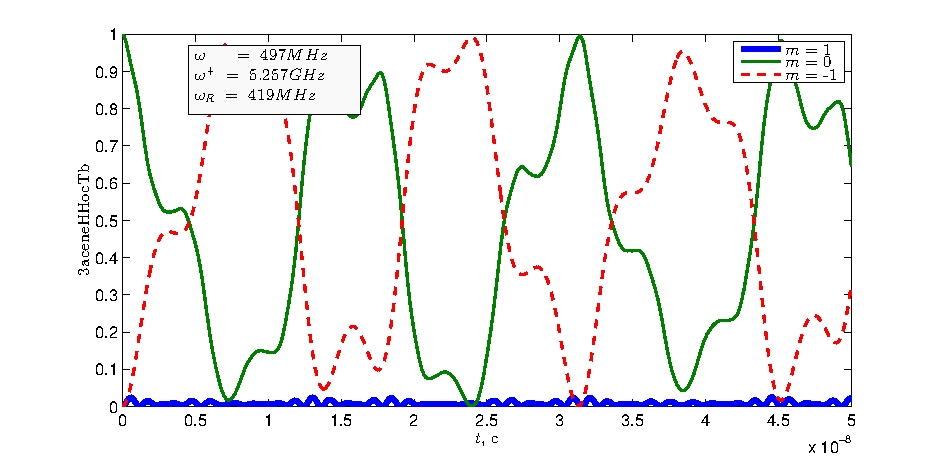
\includegraphics[width=1.1\textwidth,height=0.65\textwidth]{850_150}
  \caption{Эволюция заселенностей уровней NV-центра.}\label{fig:850_150}
\end{figure}

Можно видеть, что при дальнейшем увеличение частоты Раби, паразитная
заселенность уровня с проекцией спина $m_s$=$-1$ возрастает настолько
сильно(\ref{fig:350_300}), (\ref{fig:850_680}), что говорить об успешных
однокубитных операциях не приходится. На графиках представлены расчеты
с параметрами задачи: постоянное 350 Гс, переменное -- 300 Гс и
постоянное поле 850 Гс, переменно -- 680 Гс соответственно.
\begin{figure}[h!]\centering
  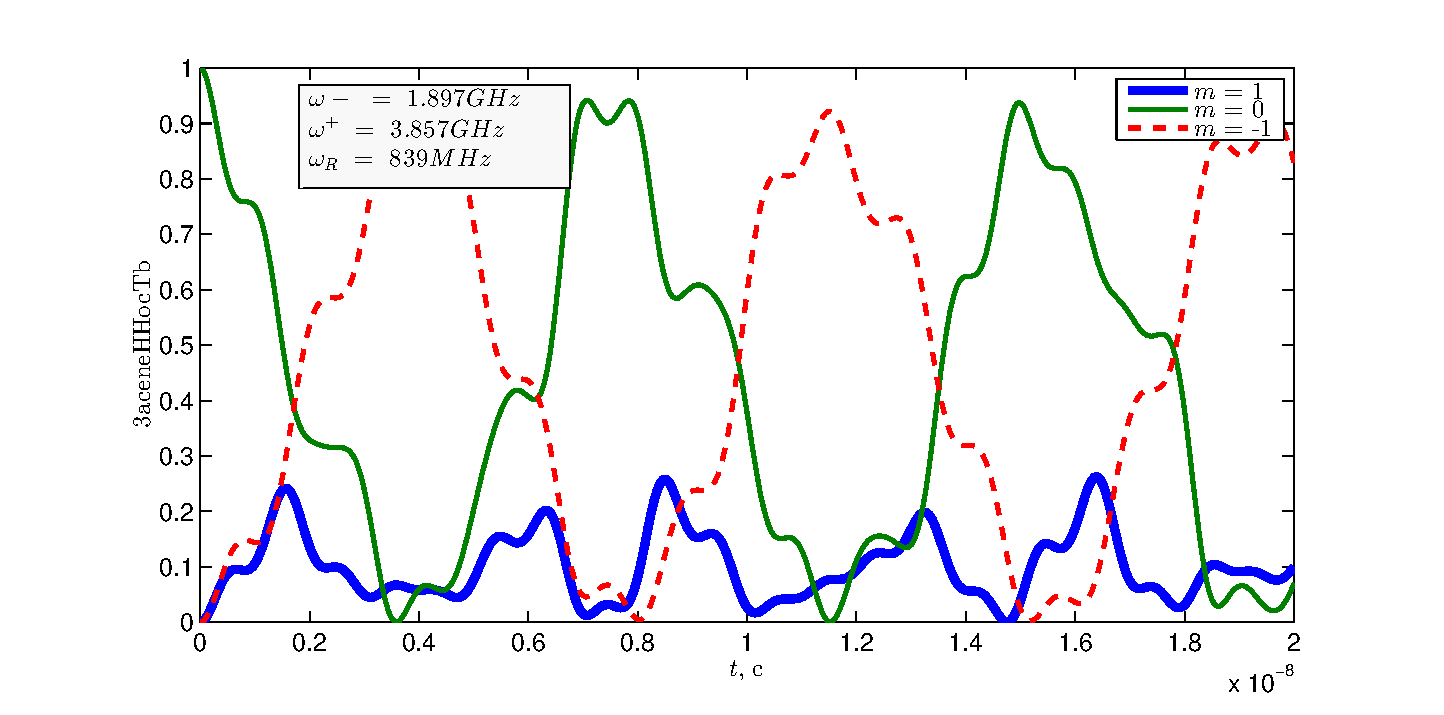
\includegraphics[width=1.1\textwidth,height=0.63\textwidth]{350_300}
  \caption{Эволюция заселенностей уровней NV-центра.}\label{fig:350_300}
\end{figure}
\begin{figure}[h!]\centering
  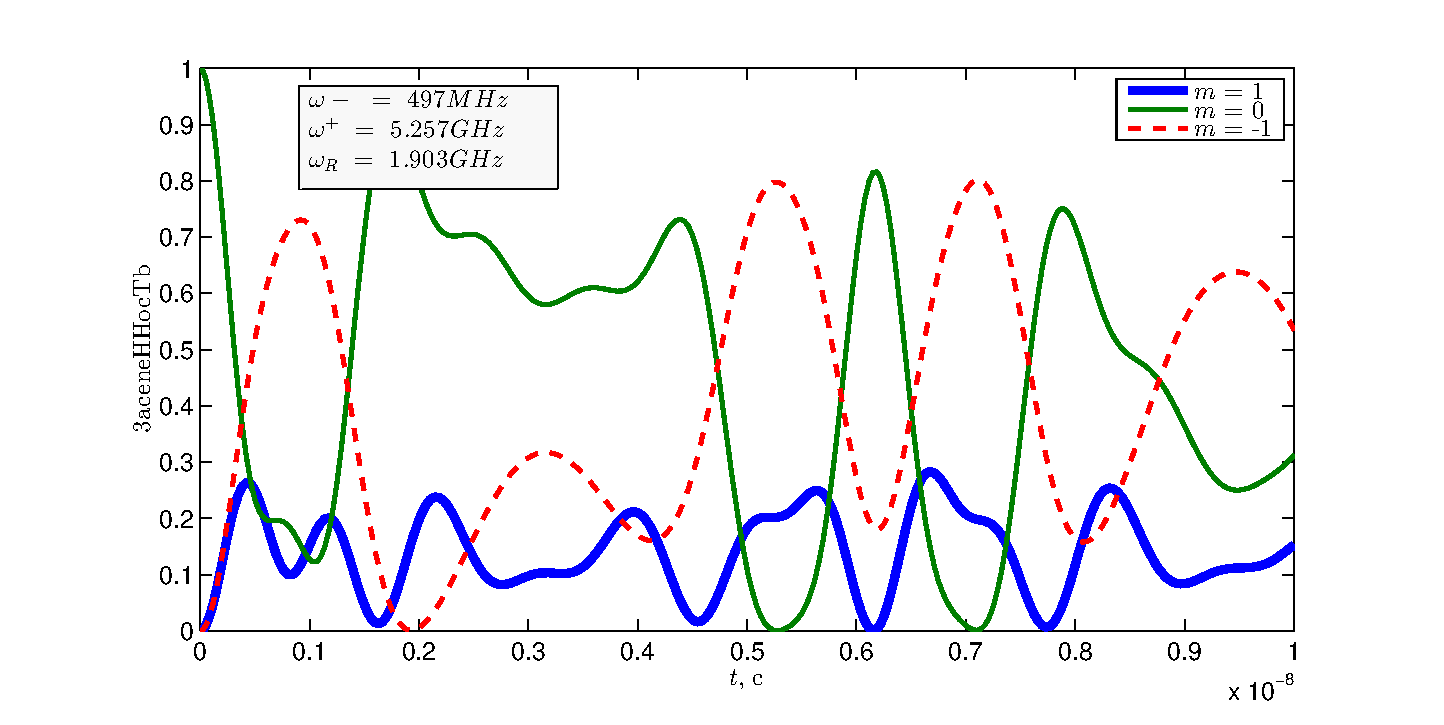
\includegraphics[width=1.1\textwidth,height=0.6\textwidth]{850_680}
  \caption{Эволюция заселенностей уровней NV-центра.}\label{fig:850_680}
\end{figure}

Из графиков (\ref{fig:350_30}) - (\ref{fig:850_680}) видно, что скорость
операции NOT возрастает с увеличением частоты Раби. Исходя из этого
соображения частота Раби была выбрана такой, чтобы паразитная
заселенность оставалась очень малой, а скорость операции была
максимальна. Чтобы еще более ускорить операцию, было произведено
варьирование формы амплитуды микроволнового импульса.

Постоянное поле было выбрано амплитудой 850 Гс, переменное -
170 Гс. Расчеты произведены для различных форм амплитуды: прямоугольные
импульсы (\ref{fig:850_170}), импульсы в форме гауссиана
(\ref{fig:gauss}) и пилообразные импульсы (\ref{fig:saw}).
\begin{figure}[H]\centering
  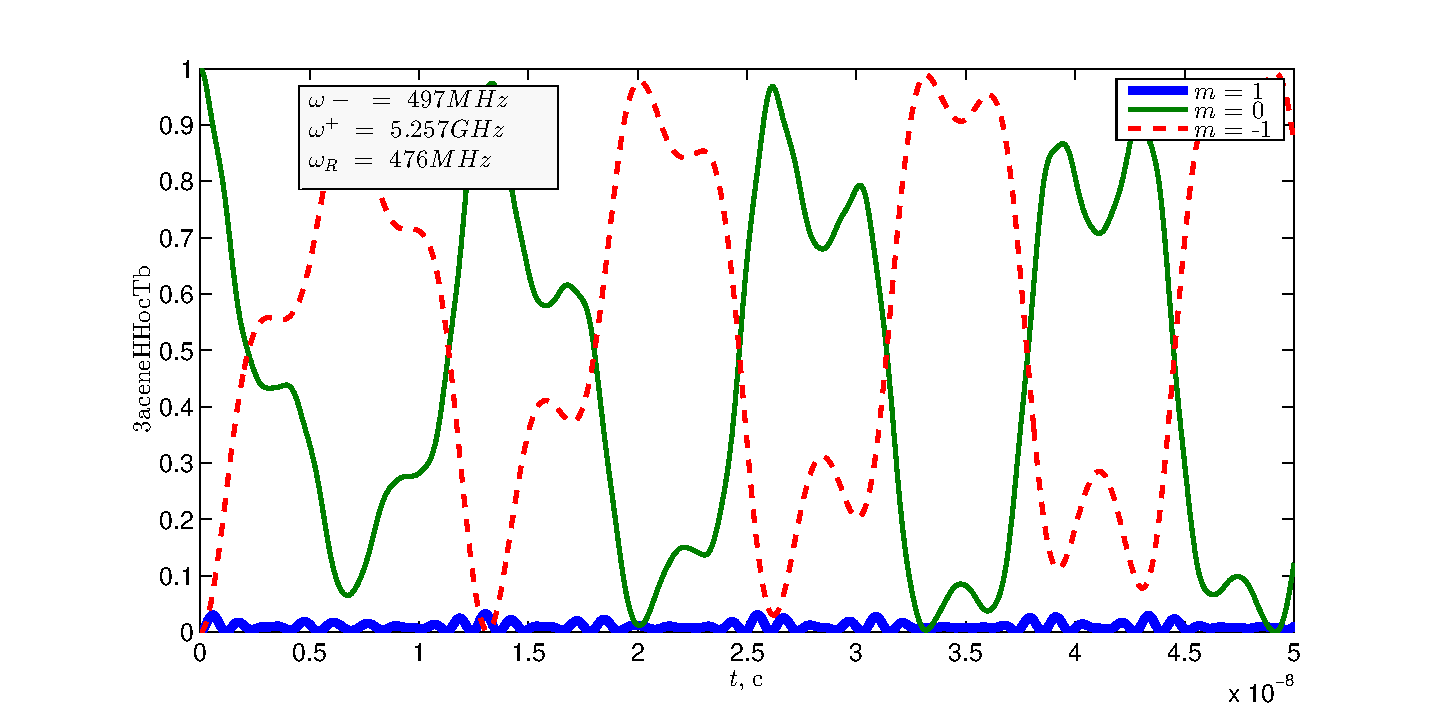
\includegraphics[width=1.1\textwidth,height=0.6\textwidth]{850_170}
  \caption{Эволюция заселенностей уровней NV-центра. Прямоугольные импульсы.}\label{fig:850_170}
\end{figure}
\begin{figure}[H]\centering
  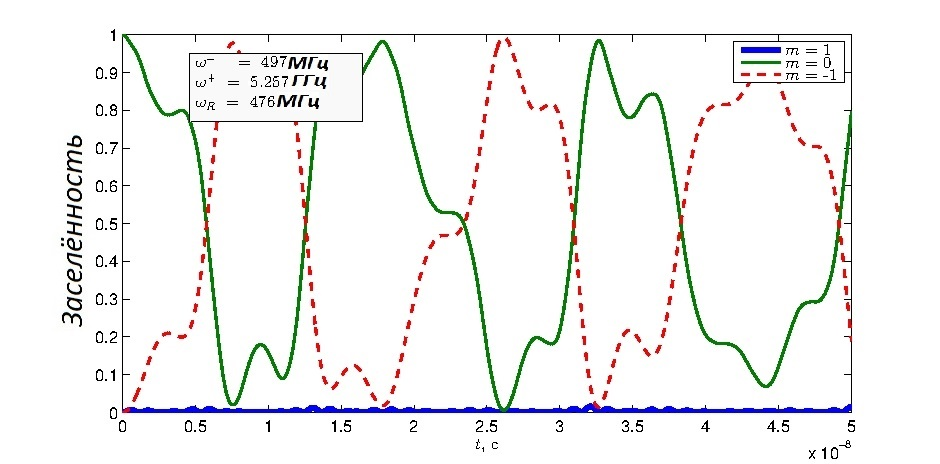
\includegraphics[width=1.1\textwidth,height=0.65\textwidth]{gauss}
  \caption{Эволюция заселенностей уровней NV-центра. Импульсы в форме гауссиана.}\label{fig:gauss}
\end{figure}
\begin{figure}[H]\centering
  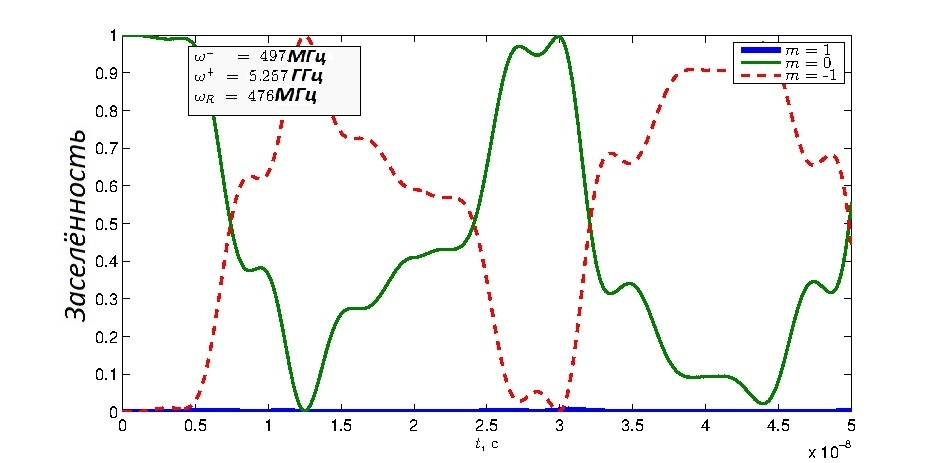
\includegraphics[width=1.1\textwidth,height=0.61\textwidth]{saw}
  \caption{Эволюция заселенностей уровней NV-центра. Пилообразные импульсы.}\label{fig:saw}
\end{figure}

Как видно из графиков (\ref{fig:850_170}) - (\ref{fig:saw}), наиболее
быстрой оказывается операция NOT, произведенная под воздействием
импульсов в форме гауссиана.

На графике (\ref{fig:850_170}) в районе 6 нс видна операция NOT, но
вероятность ее осуществления только около 95\%, а в районе 14 нс
вероятность осуществления операции стремится к 100\%. В то время как
на графике (\ref{fig:gauss}) в районе 7 нс видна операция NOT с
вероятностью около 99\%.

В работе [\ref{lit:gigahertz}] были получены еще более впечатляющие
результаты. Авторы демонстрируют наносекундные операции NOT. В их
расчетах использовалось постоянное поле 850 Гс и переменное поле на
резонансной частоте. На рисунке (\ref{fig:gigahertz}) показаны
результаты, полученные при различных значениях частоты Раби.
\begin{figure}[H]\centering
  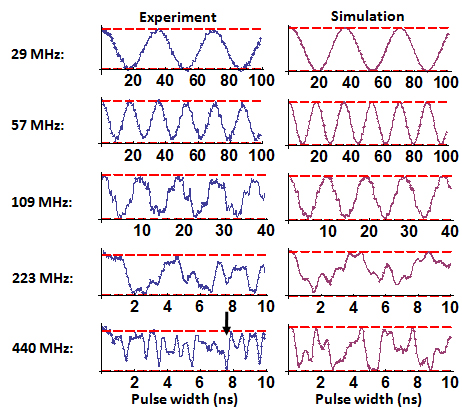
\includegraphics[height=0.9\textwidth]{gigahertz}
  \caption{``Gigahertz Dynamics of a Strongly Driven Single Quantum
  Spin''. Fuchs, Dobrovitski, Toyli, Heremans, Awschalom.}\label{fig:gigahertz}
\end{figure}

Можно видеть сильную ангармоничность заселенностей в сильных
переменных полях. При частоте Раби, равной 440 МГц, получены наиболее
быстрые осцилляции.

Моделирование системы при тех же условиях, что в работе
[\ref{lit:gigahertz}] при частоте Раби 440 МГц, показало, что
результаты, полученные в данной работе, в целом схожи с результатами
работы [\ref{lit:gigahertz}]. Однако программа (\ref{code})
демонстрирует несколько менее быстрые операции NOT. Получившиеся результаты представлены на
графике (\ref{fig:850_gigahertz}).
\begin{figure}[H]\centering
  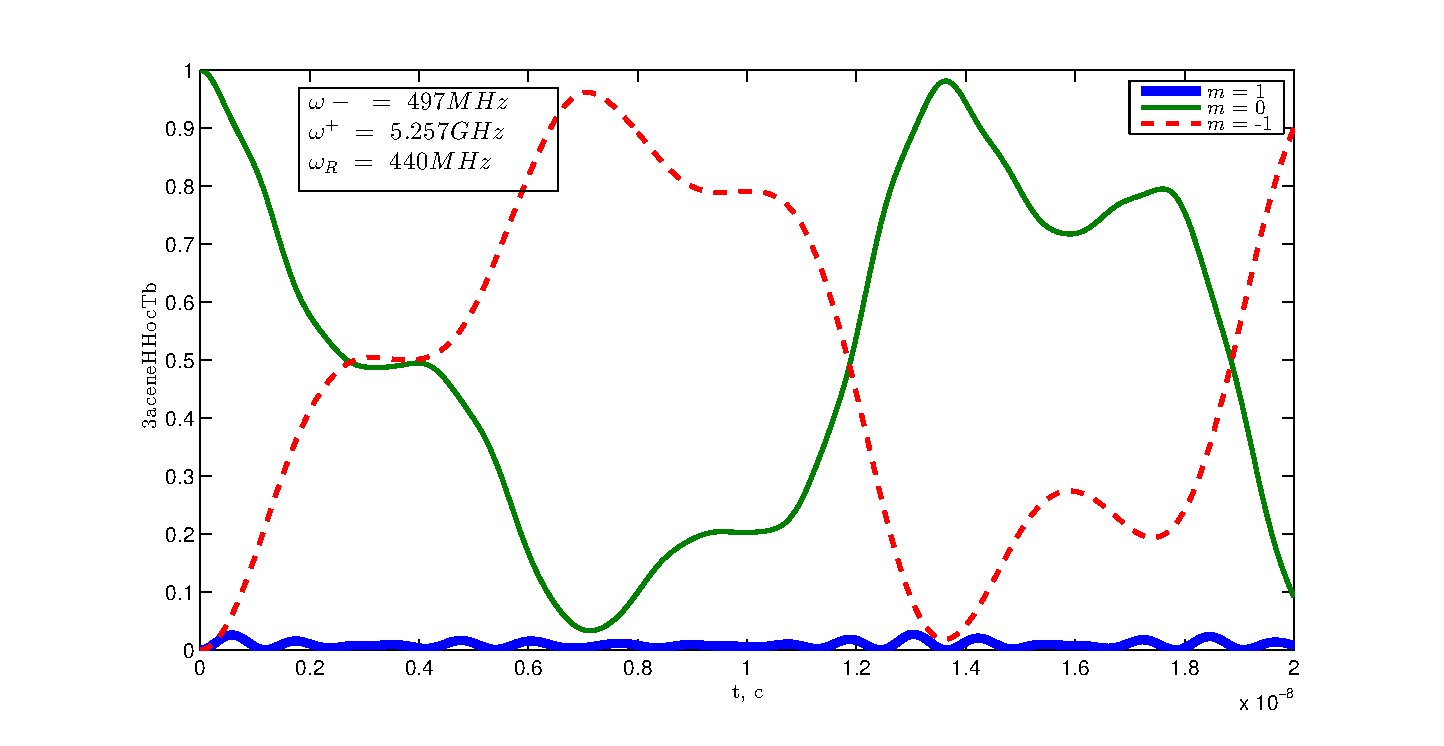
\includegraphics[width=1.1\textwidth,height=0.65\textwidth]{850_gigahertz}
  \caption{Эволюция заселенностей уровней NV-центра. Пилообразные импульсы.}\label{fig:850_gigahertz}
\end{figure}
